Dado lo que acabamos de aprender en la conferencia anterior, parecería que la atención resuelve todos los problemas con las RNN y las arquitecturas codificador-decodificador\footnote{El material siguiente se basa en: \url{http://mlexplained.com/2017/12/29/attention-is-all-you-need-explained/} y \url{http://jalammar.github.io/illustrated-transformer/}}. Sin embargo, hay algunas deficiencias de las RNN que otra arquitectura llamada \textbf{Transformer} intenta abordar. El Transformer descarta el componente recursivo de la arquitectura codificador-decodificador y se basa únicamente en los mecanismos de atención \cite{vaswani2017attention}. Cuando procesamos una secuencia con RNN, cada estado oculto depende del estado oculto anterior. Esto se convierte en un gran problema en las GPU: las GPU tienen una gran capacidad de cálculo y no les gusta tener que esperar a que los datos estén disponibles. Incluso con tecnologías como CuDNN, las RNN son dolorosamente ineficientes y lentas en la GPU.


\subsection{Dependencias en la traducción automática neuronal}
En esencia, hay tres tipos de dependencias en la traducción automática neuronal:
\begin{enumerate}
\item Dependencias entre los tokens de entrada y los tokens de salida.
\item Dependencias entre los tokens de entrada en sí.
\item Dependencias entre los tokens de salida en sí.
\end{enumerate}

El mecanismo de atención tradicional resolvió en gran medida la primera dependencia al darle al decodificador acceso a toda la secuencia de entrada. Las dependencias segunda y tercera fueron abordadas por las RNN.

\section{El Transformer}
La idea novedosa del Transformer es extender este mecanismo para procesar las oraciones de entrada y salida también. La RNN procesa secuencias de entrada de manera secuencial. El Transformer, por otro lado, permite que el codificador y el decodificador vean toda la secuencia de entrada de una vez. Esto se logra mediante la atención.

Comencemos por ver el Transformer como una caja negra única. En una aplicación de traducción automática, tomaría una oración en un idioma y produciría su traducción en otro.


\begin{figure}[h]
  \centering
  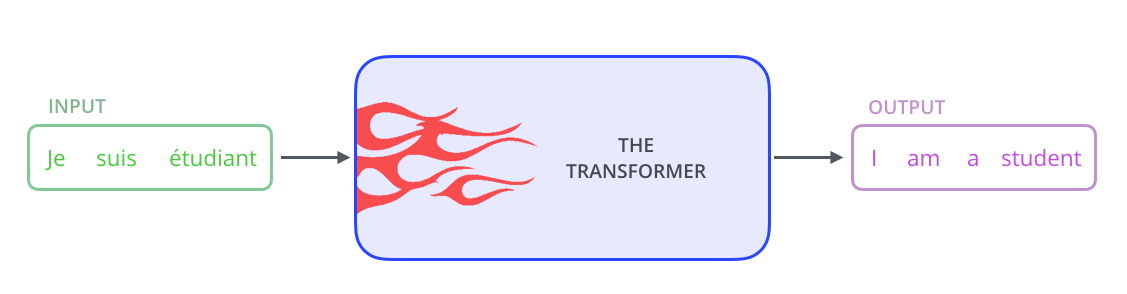
\includegraphics[scale=0.29]{pics/the_transformer_3.png}
  \caption{El Transformer como una caja negra única.}
\end{figure}

Esta caja negra se puede descomponer en un componente de codificación, un componente de decodificación y conexiones entre ellos.
\begin{figure}[h]
  \centering
  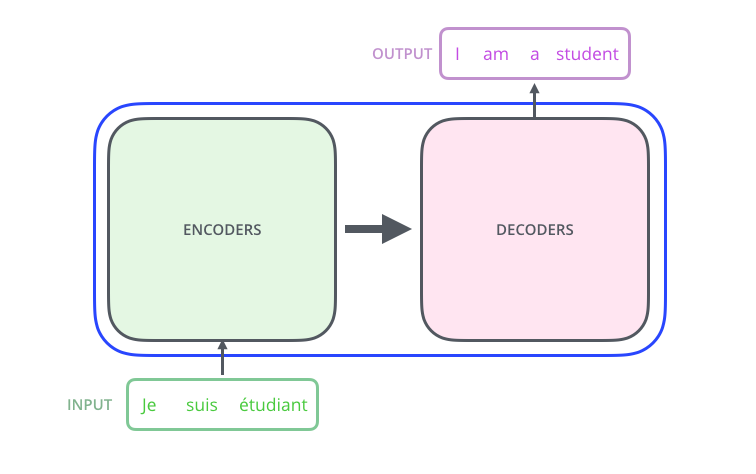
\includegraphics[scale=0.29]{pics/The_transformer_encoders_decoders.png}
  \caption{El Transformer descompuesto en componentes de codificación y decodificación.}
\end{figure}

El componente de codificación es una pila de codificadores. El Transformer original apila seis de ellos uno encima del otro. Pero no hay nada mágico en el número seis, definitivamente se pueden experimentar con otros arreglos. El componente de decodificación es una pila de decodificadores del mismo número.

\begin{figure}[h]
  \centering
  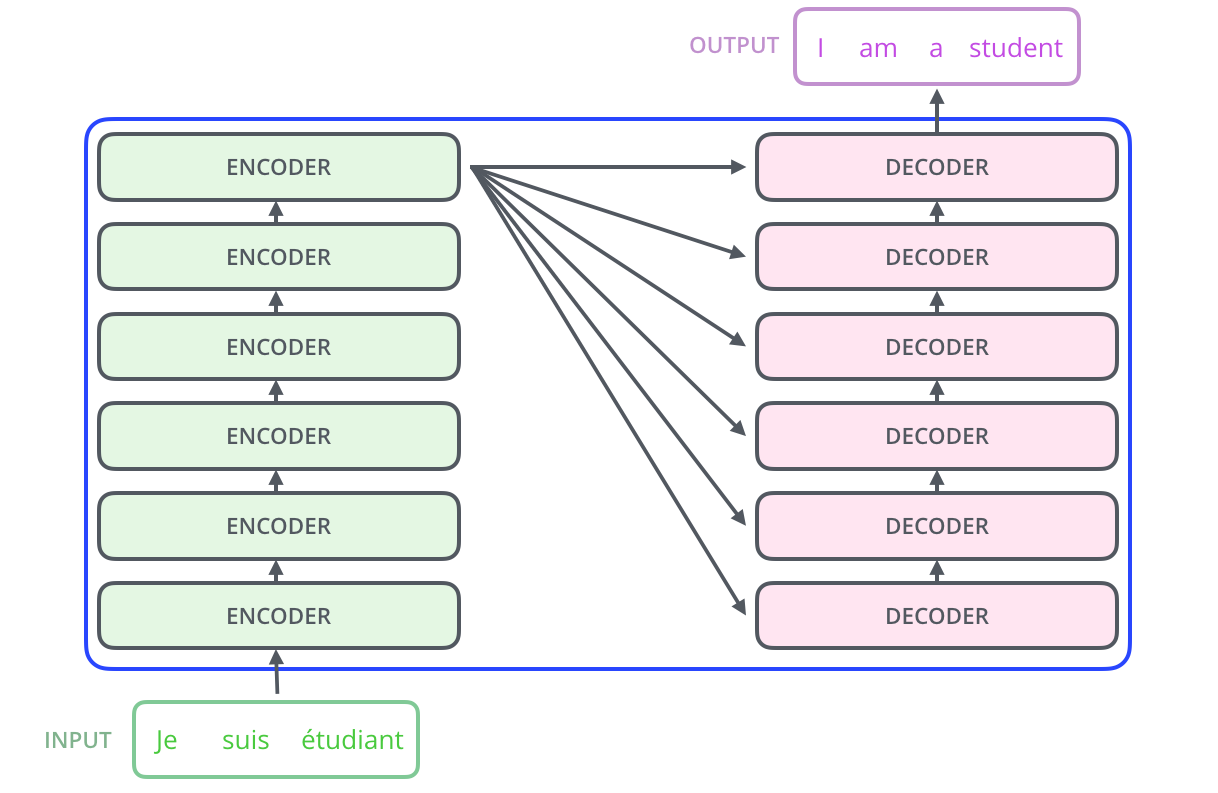
\includegraphics[scale=0.2]{pics/The_transformer_encoder_decoder_stack.png}
  \caption{Pila de codificadores y decodificadores del Transformer.}
\end{figure}
\begin{figure}[h]
  \centering
  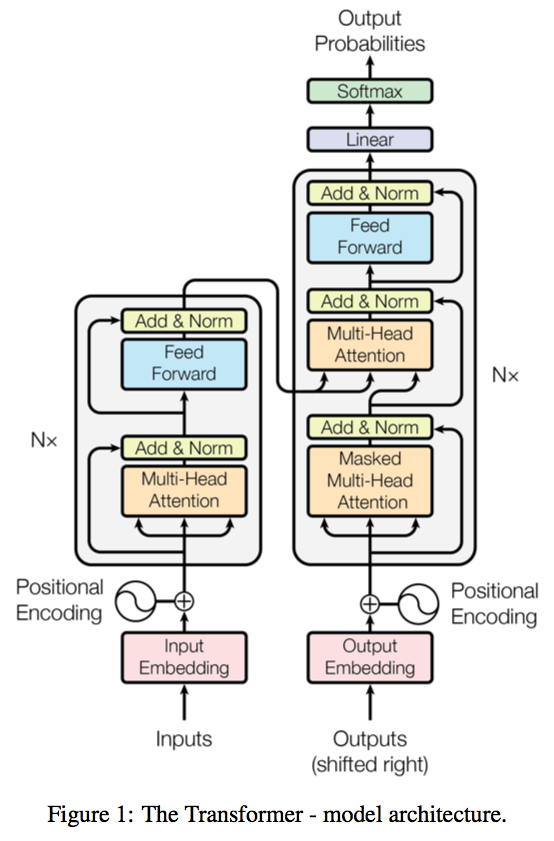
\includegraphics[scale=0.29]{pics/transformer.png}
  \caption{Estructura general del Transformer.}
\end{figure}

El Transformer todavía utiliza el diseño codificador-decodificador básico de los sistemas de traducción automática neuronal RNN. El lado izquierdo es el codificador y el lado derecho es el decodificador. Las entradas iniciales al codificador son las incrustaciones de la secuencia de entrada. Las entradas iniciales al decodificador son las incrustaciones de las salidas hasta ese momento. El codificador y el decodificador están compuestos por $N$ bloques (donde $N = 6$ para ambas redes).  Estos bloques también están compuestos por bloques más pequeños. Antes de examinar cada bloque con más detalle, intentemos comprender el mecanismo de atención implementado por el Transformer.

\section{Mecanismo de atención en el Transformer}
El mecanismo de atención en el Transformer se interpreta como una forma de calcular la relevancia de un conjunto de \textbf{valores} (información) en función de algunas \textbf{claves} y \textbf{consultas}. El mecanismo de atención se utiliza como una forma para que el modelo \textbf{se centre en la información relevante} según lo que está procesando actualmente. En la arquitectura codificador-decodificador RNN con atención:
  \begin{enumerate}
    \item Los pesos de atención eran la relevancia de los estados ocultos del codificador (valores) en el procesamiento del estado del decodificador (consulta).
    \item Estos valores se calcularon en función de los estados ocultos del codificador (claves) y el estado oculto del decodificador (consulta).
  \end{enumerate}

\begin{figure}[h]
  \centering
  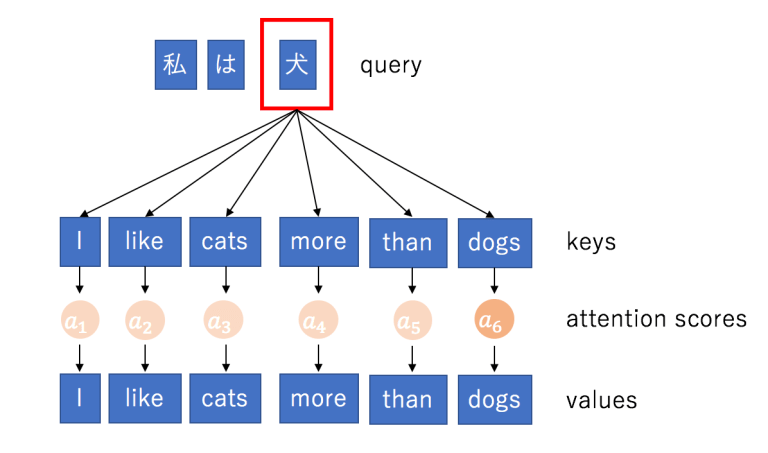
\includegraphics[scale=0.2]{pics/attention_concept.png}
  \caption{Concepto de atención en el Transformer.}
\end{figure}

En este ejemplo, la consulta es la palabra que se está decodificando (lo cual significa ``perro'') y tanto las claves como los valores son la oración fuente. El puntaje de atención representa la relevancia y, en este caso, es alto para la palabra ``perro'' y bajo para las demás. Cuando pensamos en la atención de esta manera, podemos ver que las claves, valores y consultas podrían ser cualquier cosa. Incluso podrían ser iguales. Por ejemplo, tanto los valores como las consultas podrían ser las incrustaciones de entrada (autoatención).


\subsection{Consultas}
Las consultas son representaciones de la secuencia de destino o salida que el modelo Transformer utiliza para determinar cuánta atención se debe prestar a cada palabra en la secuencia de entrada. Cada palabra o token en la secuencia de salida se asocia con una consulta. Las consultas ayudan a recuperar la información relevante de la secuencia de entrada. Ejemplo: Si estamos generando la traducción para la oración ``Je adore les chats'' (que significa ``Me encantan los gatos'' en francés), cada palabra en la secuencia de salida tendría su representación de consulta correspondiente. Por ejemplo, ``Je'' tendría un vector de consulta, ``adore'' tendría un vector de consulta, y así sucesivamente.

\subsection{Claves}
Las claves son representaciones de la secuencia de entrada que el modelo Transformer utiliza para calcular los puntajes de atención. Cada palabra o token en la secuencia de entrada se asocia con una clave. Estas claves capturan la información necesaria para comprender el contexto y las relaciones entre las palabras de la secuencia.
Ejemplo: Consideremos la secuencia de entrada: ``I love cats'' (Amo a los gatos). Cada palabra en la secuencia tendría su representación de clave correspondiente, como ``I'' teniendo un vector de clave, ``love'' teniendo un vector de clave, y así sucesivamente.

\subsection{Valores}
Los valores son la información o características reales asociadas con cada palabra de la secuencia de entrada. Estos valores se utilizan para calcular la suma ponderada durante el cálculo de la atención, lo que ayuda a determinar la importancia o relevancia de cada palabra. Ejemplo: Considerando la misma secuencia de entrada ``I love cats'', cada palabra tendría su representación de valor asociada. Estos valores contienen la información contextual para cada palabra. Por ejemplo, ``I'' tendría un vector de valor, ``love'' tendría un vector de valor, y así sucesivamente.
Las claves y los valores son muy difíciles de distinguir a primera vista porque en la codificación y decodificación RNN con atención clásica son iguales. Veremos con el Transformer que aunque provienen de la misma secuencia, pueden corresponder a vectores diferentes.


\subsection{Atención de producto puntual escalado}
El Transformer utiliza una forma particular de atención llamada ``Atención de Producto Puntual Escalado''. Para un vector de consulta dado $\vec{q}$, una secuencia de vectores clave $\vec{k}_{1:m}$ y una secuencia de vectores valor $\vec{v}_{1:m}$, los pesos de atención $\alpha_1,\dots,\alpha_m$ se calculan de la siguiente manera:
\begin{displaymath}
\alpha_1,\dots,\alpha_m = \text{softmax}\left(\frac{\vec{q} \cdot \vec{k}_{1}}{\sqrt{d}}, \dots,\frac{\vec{q} \cdot \vec{k}_{1}}{\sqrt{d}}\right)
\end{displaymath}
$d$ representa la dimensionalidad de las consultas y las claves.

La normalización sobre $\sqrt{d}$ se utiliza para reescalar los productos punto entre consultas y claves (los productos punto tienden a crecer con la dimensionalidad). Los pesos de atención se multiplican entonces por sus valores correspondientes para calcular una suma ponderada, que luego se pasa a las capas subsiguientes de la red:

\begin{displaymath}
\alpha_1*\vec{v}_1+\cdots+\alpha_m*\vec{v}_m
\end{displaymath}

Ahora estamos listos para analizar más de cerca cada parte del Transformer.

\section{El Codificador}
El codificador contiene capas de autoatención.

En una capa de autoatención, todas las claves, valores y consultas provienen del mismo lugar, en este caso, la salida de la capa anterior en el codificador.

Cada posición en el codificador puede atender a todas las posiciones en la capa anterior del codificador.

El codificador está compuesto por dos bloques (que llamaremos subcapas para distinguirlos de los $N$ bloques que componen el codificador y el decodificador).

Uno es la subcapa de atención multihead sobre las entradas, mencionada anteriormente.

El otro es una red neuronal de alimentación directa simple.

\begin{figure}[h]
\centering
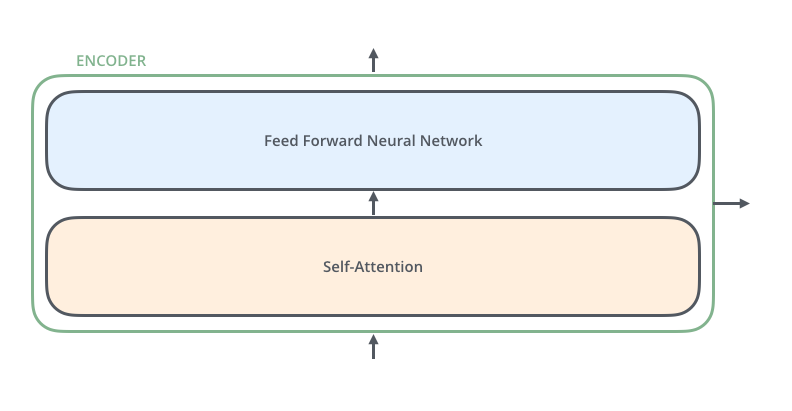
\includegraphics[scale=0.35]{pics/Transformer_encoder.png}
\caption{Estructura del codificador del Transformer.}
\end{figure}


\begin{figure}[h]
\centering
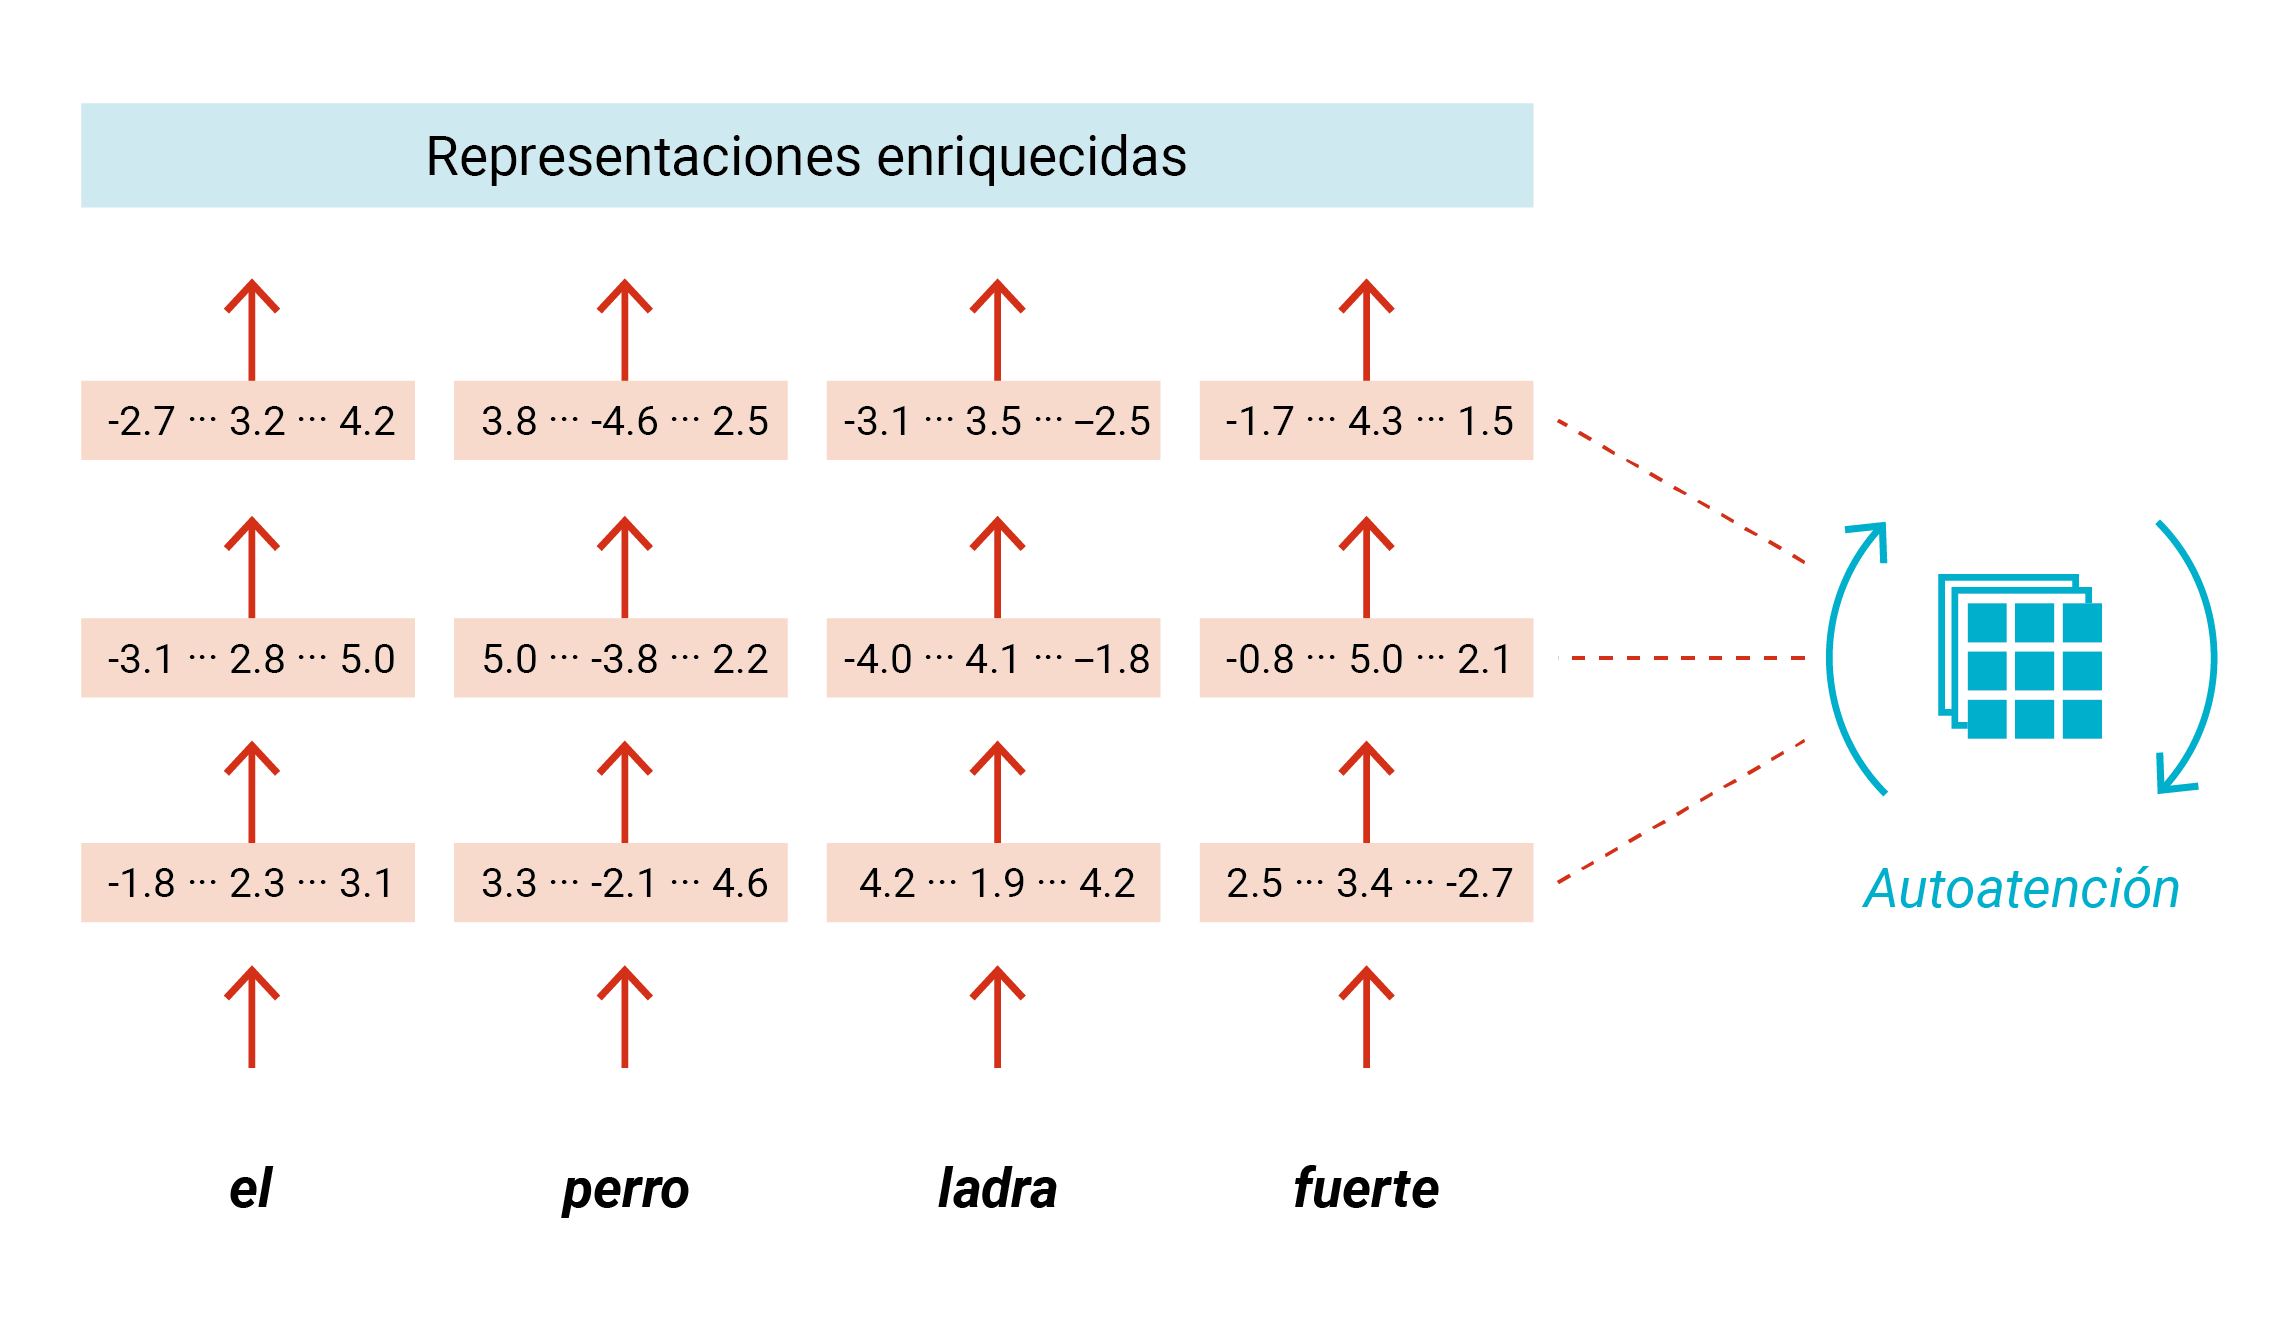
\includegraphics[scale=0.6]{pics/selfattention.png}
\caption{Idea general del proceso de auto-atención.}
\end{figure}

\paragraph{Introduciendo los tensores en la imagen}
Comenzamos convirtiendo cada palabra de entrada en un vector utilizando una capa de incrustación de tamaño 512 en el codificador más inferior.
\begin{figure}[h]
\centering
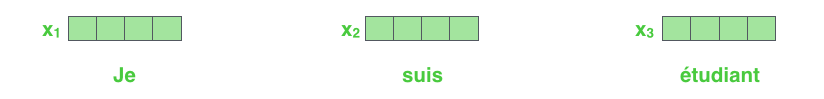
\includegraphics[scale=0.35]{pics/embeddings_enc.png}
\caption{Capa de incrustación en el codificador.}
\end{figure}

En el codificador inferior, esto serían las incrustaciones de palabras, pero en otros codificadores, sería la salida del codificador que está directamente debajo. El tamaño de esta lista es un hiperparámetro que podemos establecer: básicamente sería la longitud de la oración más larga en nuestro conjunto de datos de entrenamiento.

\begin{figure}[h]
\centering
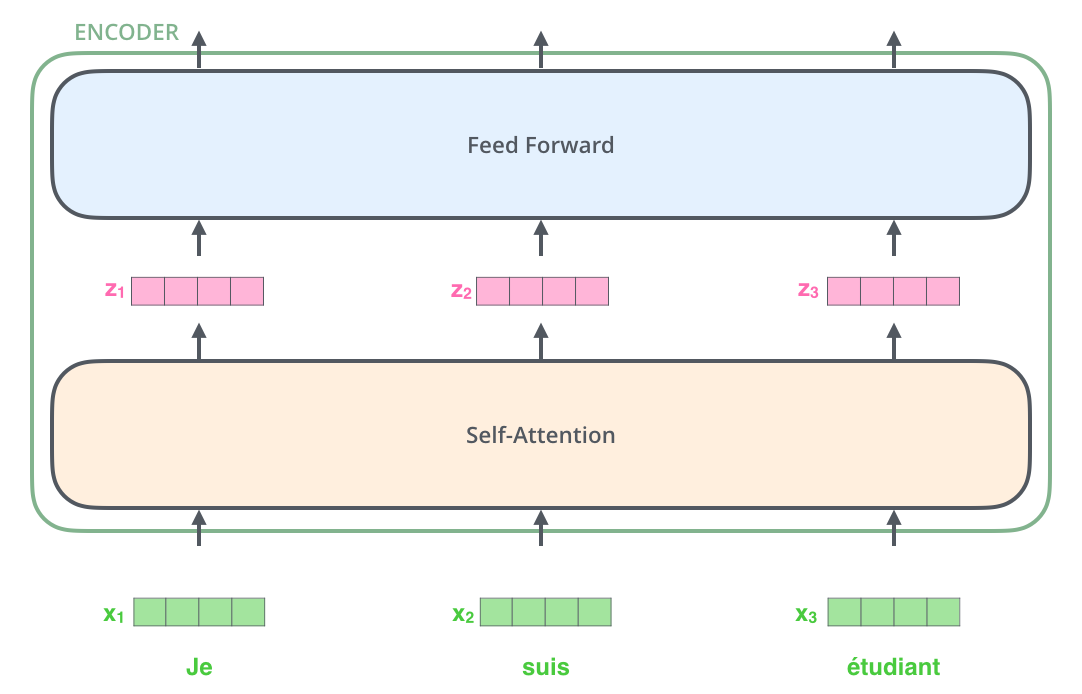
\includegraphics[scale=0.2]{pics/encoder_with_tensors.png}
\caption{Representación de las incrustaciones y los vectores de entrada en el codificador.}
\end{figure}

La palabra en cada posición fluye a través de su propio camino en el codificador. Hay dependencias entre estos caminos en la capa de autoatención. La capa de alimentación directa no tiene esas dependencias. Por lo tanto, los diversos caminos pueden ejecutarse en paralelo mientras fluyen a través de la capa de alimentación directa.
¡Ahora estamos codificando! Como hemos mencionado anteriormente, un codificador recibe una lista de vectores como entrada. Procesa esta lista pasando estos vectores a una capa de ``autoatención'', luego a una red neuronal de alimentación directa, y luego envía la salida hacia arriba al siguiente codificador.


\begin{figure}[h]
\centering
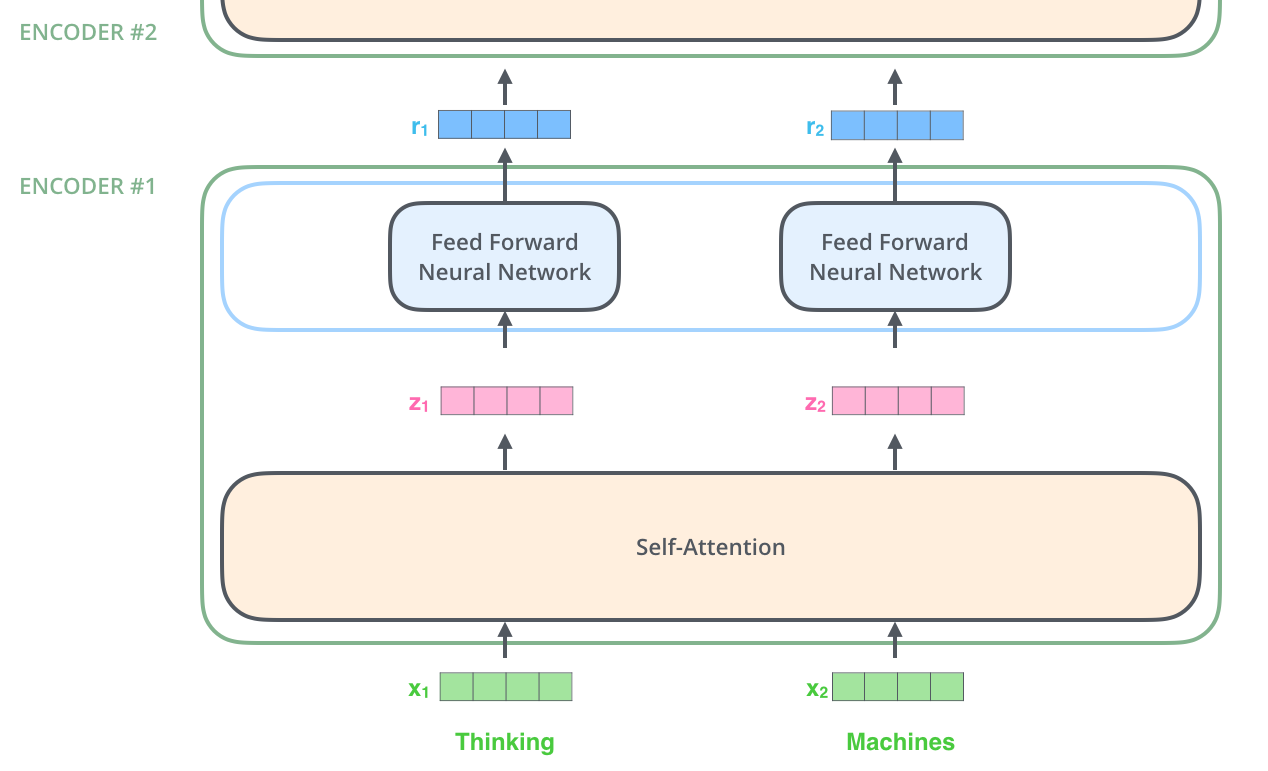
\includegraphics[scale=0.2]{pics/encoder_with_tensors_2.png}
\caption{Flujo de datos en el codificador del Transformer.}
\end{figure}


\section{Autoatención a alto nivel}

Supongamos que la siguiente oración es una oración de entrada que queremos traducir:
\\ \textcolor{red}{``The animal didn't cross the street because it was too tired''}

¿A qué se refiere ``it'' en esta oración?

¿Se refiere a la calle o al animal? No es una pregunta tan simple para un algoritmo como lo es para un humano.

Cuando el modelo está procesando la palabra ``it'', la autoatención le permite asociarla con ``animal''.

A medida que el modelo procesa cada palabra (cada posición en la secuencia de entrada), la autoatención le permite examinar otras posiciones en la secuencia de entrada en busca de pistas que puedan ayudar a obtener una mejor codificación para esta palabra.

Piense en cómo mantener un estado oculto permite que una RNN incorpore su representación de palabras/vectores anteriores que ha procesado con la palabra actual que está procesando. La autoatención es el método que el Transformer utiliza para integrar la ``comprensión'' de otras palabras relevantes en la que estamos procesando actualmente.

\begin{figure}[h]
  \centering
  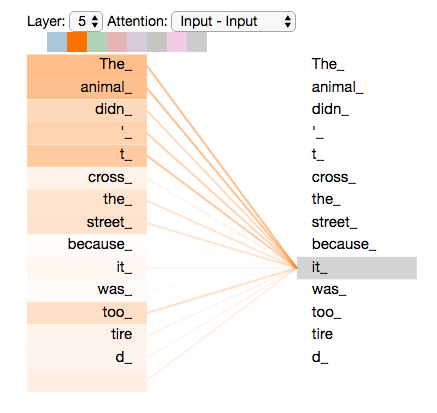
\includegraphics[scale=0.35]{pics/transformer_self-attention_visualization.png}
  \caption{Visualización de la autoatención en el Transformer.}
\end{figure}

\section{Autoatención en detalle}


\paragraph{Paso 1}

El \textbf{primer paso} para calcular la autoatención con producto puntual escalado consiste en crear tres vectores a partir de cada uno de los vectores de entrada del codificador (en este caso, la incrustación de cada palabra).

Para cada palabra, creamos un vector de consulta (\textcolor{purple}{Query}), un vector clave (\textcolor{orange}{Key}) y un vector de valor (\textcolor{blue}{Value}).

Estos vectores se crean multiplicando la incrustación por tres matrices que hemos entrenado durante el proceso de entrenamiento.

Observa que estos nuevos vectores son de menor dimensión que el vector de incrustación. Su dimensionalidad es de 64, mientras que los vectores de entrada/salida del codificador tienen una dimensionalidad de 512. No es necesario que sean más pequeños, esta es una elección arquitectónica para hacer que el cálculo de la atención multihead sea (en su mayoría) constante.

\begin{figure}[h]
  \centering
  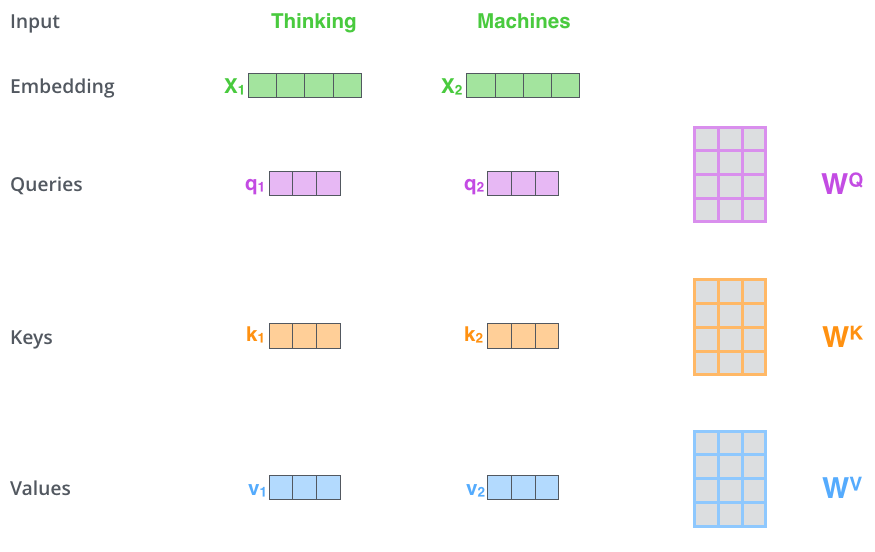
\includegraphics[scale=0.3]{pics/transformer_self_attention_vectors.png}
\end{figure}

Por ejemplo, en la oración "Thinking Machines", al multiplicar \textcolor{green}{$x_1$} por la matriz de pesos \textcolor{purple}{WQ} se obtiene el vector \textcolor{purple}{$q_1$}, que es el vector de "consulta" asociado a esa palabra. De esta manera, creamos una proyección de "consulta", "clave" y "valor" para cada palabra de la oración de entrada.

\paragraph{Paso 2}

El \textbf{segundo paso} para calcular la autoatención es calcular una puntuación.

Supongamos que estamos calculando la autoatención para la primera palabra en este ejemplo, "Thinking". Necesitamos puntuar cada palabra de la oración de entrada en relación con esta palabra. La puntuación determina cuánto enfoque debemos poner en otras partes de la oración de entrada a medida que codificamos una palabra en una posición determinada.

La puntuación se calcula tomando el producto punto del vector de "consulta" (\textcolor{purple}{Query}) con el vector de "clave" (\textcolor{orange}{Key}) de la palabra correspondiente que estamos puntuando. Por lo tanto, si estamos procesando la autoatención para la palabra en la posición \textcolor{green}{\#1}, la primera puntuación sería el producto punto de \textcolor{purple}{q1} y \textcolor{orange}{k1}. La segunda puntuación sería el producto punto de \textcolor{purple}{q1} y \textcolor{orange}{k2}.

\begin{figure}[h]
  \centering
  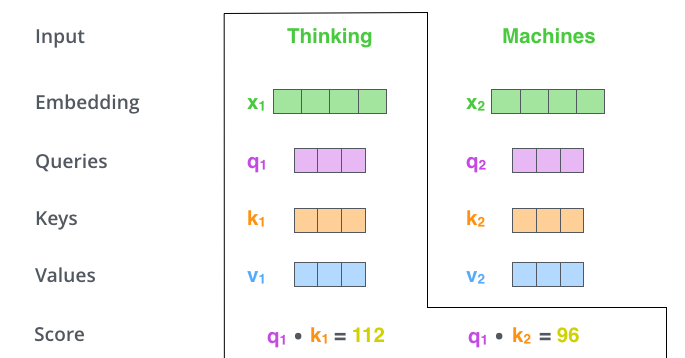
\includegraphics[scale=0.4]{pics/transformer_self_attention_score.png}
\end{figure}

\paragraph{Pasos 3 y 4}

Los \textbf{tercer} y \textbf{cuarto} pasos consisten en dividir las puntuaciones por 8 (la raíz cuadrada de la dimensión de los vectores clave utilizados en el artículo, es decir, 64).

Esto ayuda a obtener gradientes más estables. Podría haber otros posibles valores aquí, pero este es el valor por defecto. Luego, se pasa el resultado por una operación de softmax. La función softmax normaliza las puntuaciones para que sean todas positivas y sumen 1.

Estas puntuaciones de softmax determinan cuánto se expresará cada palabra en la posición actual. Claramente, la palabra en la posición actual tendrá la puntuación softmax más alta, pero a veces es útil prestar atención a otra palabra relevante para la palabra actual.

\begin{figure}[h]
  \centering
  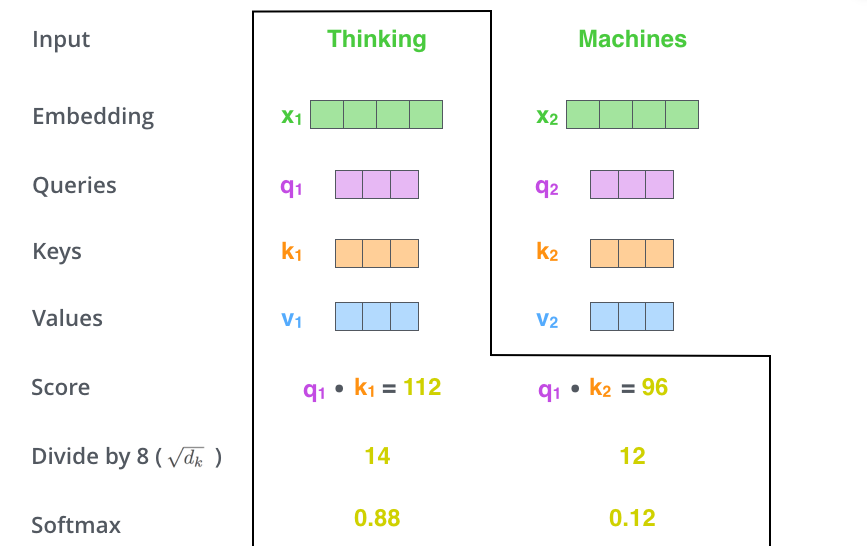
\includegraphics[scale=0.35]{pics/self-attention_softmax.png}
\end{figure}

\paragraph{Autoatención en detalle: pasos 5 y 6}

El \textbf{quinto paso} es multiplicar cada vector de valor por la puntuación softmax (en preparación para sumarlos).

La intuición aquí es mantener intactos los valores de las palabras en las que queremos enfocarnos y atenuar las palabras irrelevantes (multiplicándolas por números pequeños como 0.001, por ejemplo).

El \textbf{sexto paso} es sumar los vectores de valor ponderados. Esto produce la salida de la capa de autoatención en la posición actual (para la primera palabra en este ejemplo).

Con esto concluye el cálculo de la autoatención con producto puntual escalado. El vector resultante es el que podemos enviar a la red neuronal de avance (\textit{feed-forward neural network}).

\begin{figure}[h]
  \centering
  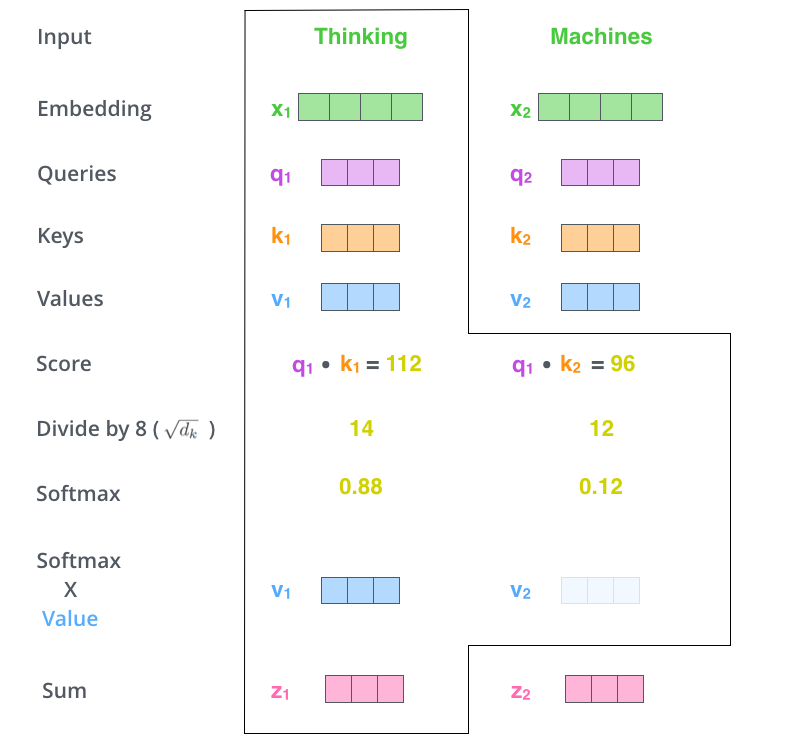
\includegraphics[scale=0.3]{pics/self-attention-output.png}
\end{figure}

\section{Cálculo matricial de la autoatención}
En la implementación real, la autoatención con producto puntual escalado se calcula en forma matricial para un procesamiento más rápido. Veamos eso ahora que hemos comprendido la intuición del cálculo a nivel de palabras. El primer paso es calcular las matrices de consulta (\textcolor{purple}{Q}), clave (\textcolor{orange}{K}) y valor (\textcolor{blue}{V}):

\begin{figure}[h]
  \centering
  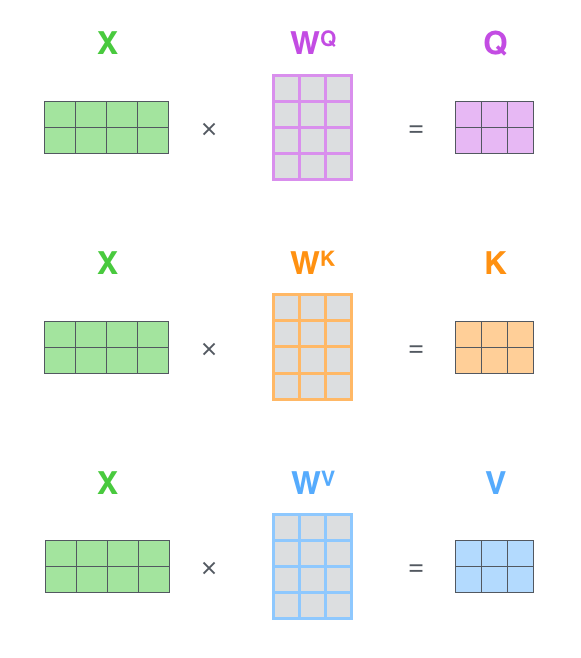
\includegraphics[scale=0.25]{pics/self-attention-matrix-calculation.png}
\end{figure}

Lo hacemos empaquetando nuestras incrustaciones en una matriz $X$ y multiplicándola por las matrices de pesos que hemos entrenado (\textcolor{purple}{WQ}, \textcolor{orange}{WK}, \textcolor{blue}{WV}).

Finalmente, como estamos tratando con matrices, podemos condensar los pasos dos a seis en una fórmula para calcular las salidas de la capa de autoatención.

\begin{figure}[h]
  \centering
  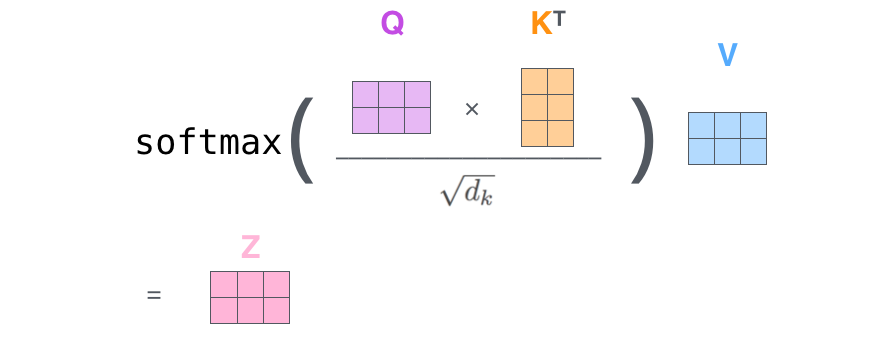
\includegraphics[scale=0.35]{pics/self-attention-matrix-calculation-2.png}
\end{figure}

        
\section{Atención multi-head}

Si solo calculáramos una única suma ponderada de atención de los valores, sería difícil capturar diferentes aspectos del input. En el ejemplo anterior, $z1$ contiene un poco de cada codificación, pero podría estar dominado por la palabra en sí misma.
Si estamos traduciendo una oración como "The animal didn't cross the street because it was too tired" (El animal no cruzó la calle porque estaba demasiado cansado), sería útil saber a qué se refiere la palabra "it" (él o ella).  Para expandir el modelo y aprender representaciones diversas centradas en diferentes posiciones, el Transformer utiliza el bloque de atención multi-head.

La atención multi-head calcula múltiples sumas ponderadas de atención en lugar de una sola pasada de atención sobre los valores. En esencia, aplica transformaciones lineales diferentes a los valores, claves y consultas para cada "head" de atención.

El bloque de atención multi-head aplica múltiples bloques de atención con producto puntual escalado en paralelo, concatena sus salidas y luego aplica una única transformación lineal.

\begin{figure}[h]
  \centering
  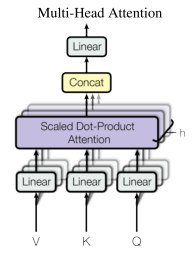
\includegraphics[scale=0.48]{pics/multi_head_attention.png}
\end{figure}

Con la atención multi-head, no tenemos uno, sino varios conjuntos de matrices de pesos de consulta/clave/valor. El Transformer utiliza ocho cabezas de atención, por lo que obtenemos ocho conjuntos para cada codificador/decodificador. Cada uno de estos conjuntos se inicializa de forma aleatoria. Luego, después del entrenamiento, cada conjunto se utiliza para proyectar las incrustaciones de entrada (o vectores de codificadores/decodificadores inferiores) en un subespacio de representación diferente. El componente de atención multi-head proporciona a la capa de atención múltiples ``subespacios de representación''

\begin{figure}[h]
  \centering
  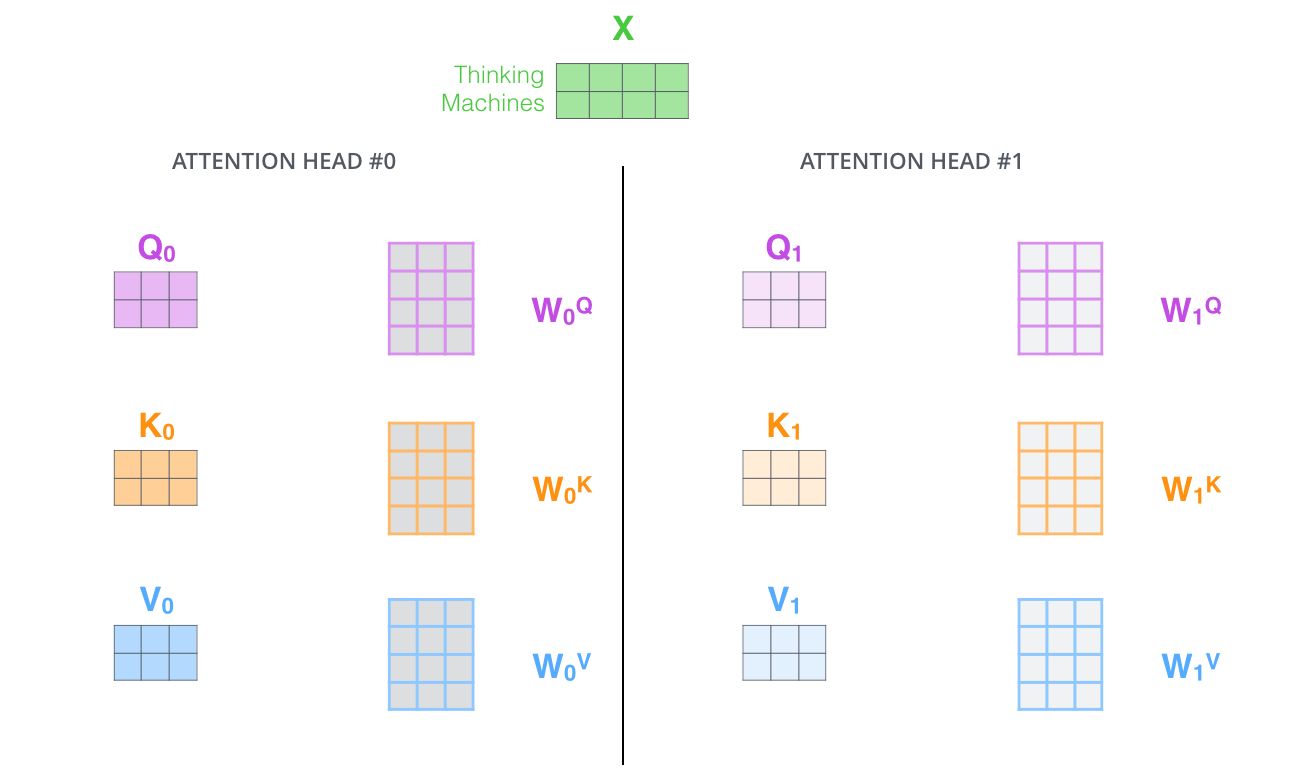
\includegraphics[scale=0.2]{pics/transformer_attention_heads_qkv.png}
\end{figure}

Con la atención multi-head, mantenemos matrices de pesos de consulta/clave/valor separadas para cada cabeza, lo que resulta en diferentes matrices de consulta/clave/valor. Como hicimos antes, multiplicamos X por las matrices WQ/WK/WV para obtener las matrices de consulta/clave/valor.

\begin{figure}[h]
  \centering
  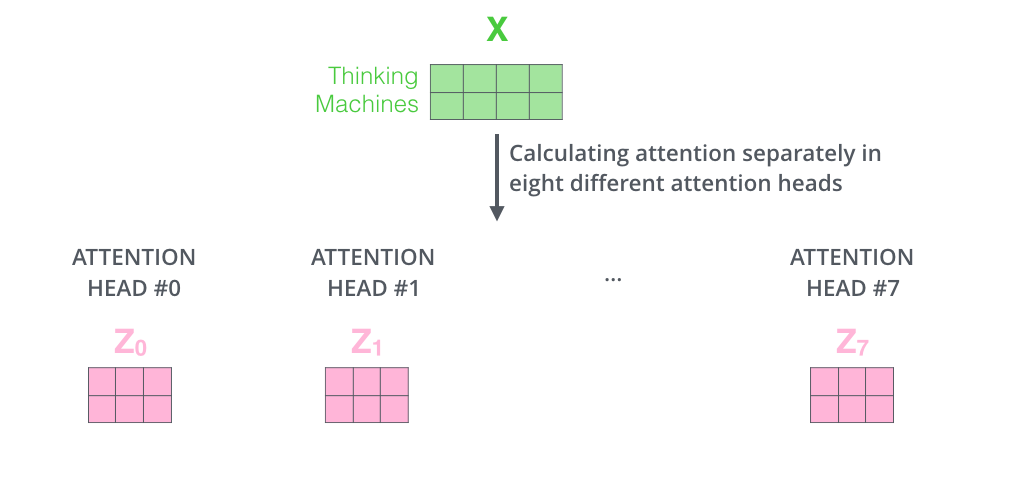
\includegraphics[scale=0.25]{pics/transformer_attention_heads_z.png}
\end{figure}

Si realizamos el mismo cálculo de autoatención que hemos descrito anteriormente, pero ocho veces diferentes con diferentes matrices de pesos, obtendremos ocho matrices Z diferentes. Sin embargo, la red de alimentación espera una única matriz (un vector para cada palabra), no ocho matrices. Entonces, necesitamos una forma de condensar estas ocho matrices en una sola matriz. Esto se logra concatenando las matrices y luego multiplicándolas por una matriz de pesos adicional WO.

\begin{figure}[h]
  \centering
  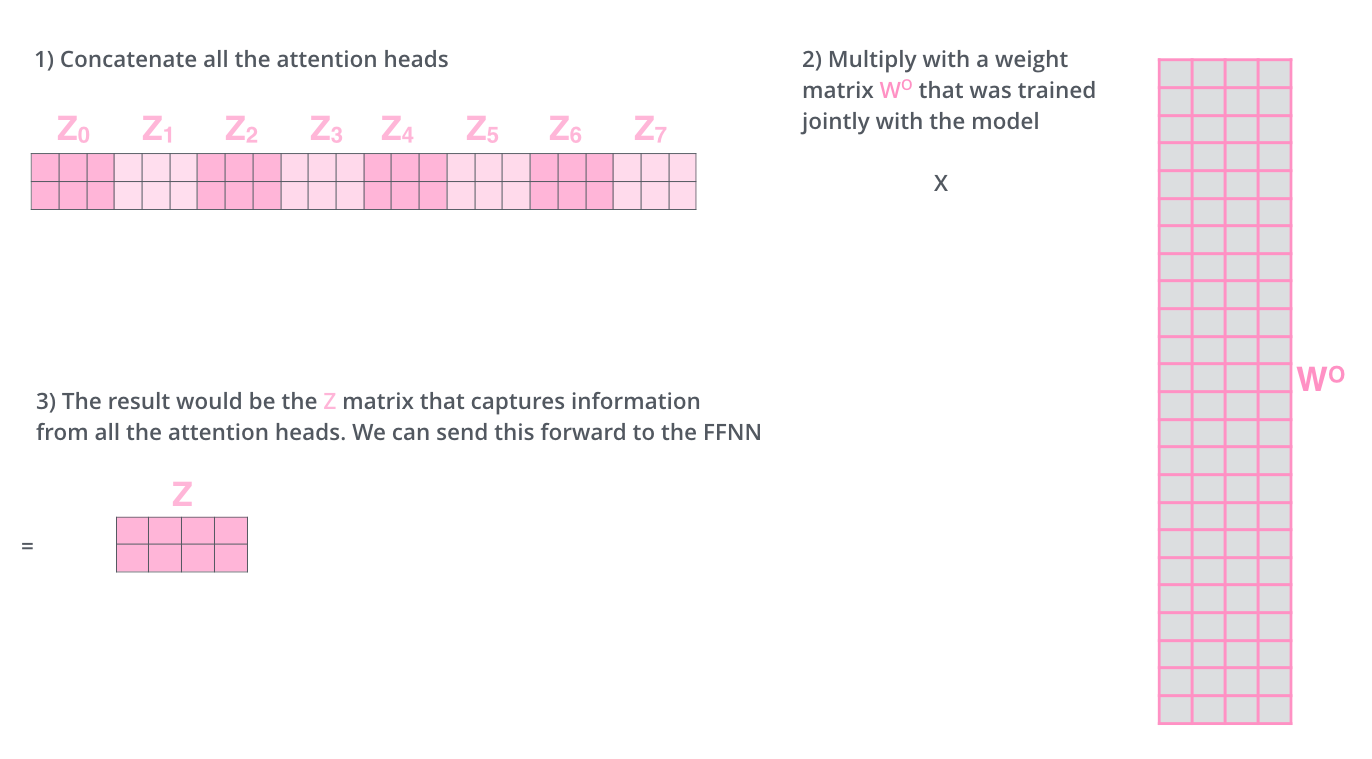
\includegraphics[scale=0.22]{pics/transformer_attention_heads_weight_matrix_o.png}
\end{figure}

Veamos todas estas matrices juntas en una visualización para poder verlas en un solo lugar.

\begin{figure}[h]
  \centering
  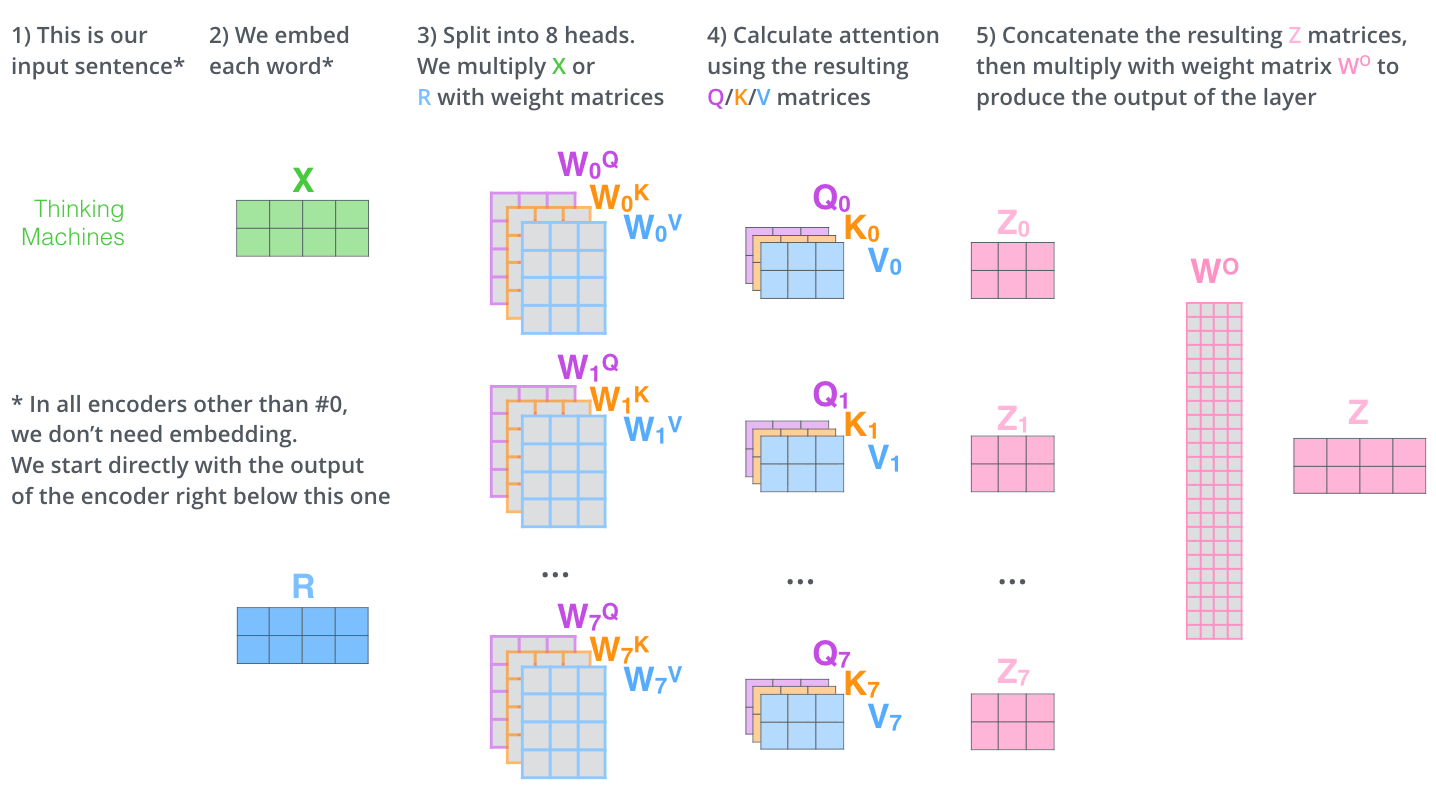
\includegraphics[scale=0.226]{pics/transformer_multi-headed_self-attention-recap.png}
\end{figure}

\section{Conexiones residuales}
Entre cada subcapa, hay una conexión residual seguida de una normalización de capa.
Una conexión residual consiste básicamente en tomar la entrada y sumarla a la salida de la subred, y es una forma de facilitar el entrenamiento de redes profundas.
La normalización de capa es un método de normalización en el aprendizaje profundo que es similar a la normalización de lote (\textit{batch normalization}).

\begin{figure}[h]
  \centering
  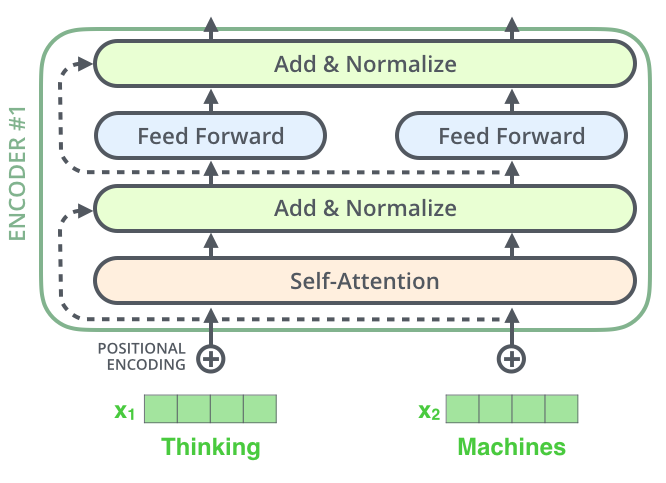
\includegraphics[scale=0.3]{pics/transformer_resideual_layer_norm.png}
\end{figure}

Si visualizamos los vectores y la operación de normalización de capa asociada con la autoatención, se vería así:

\begin{figure}[h]
  \centering
  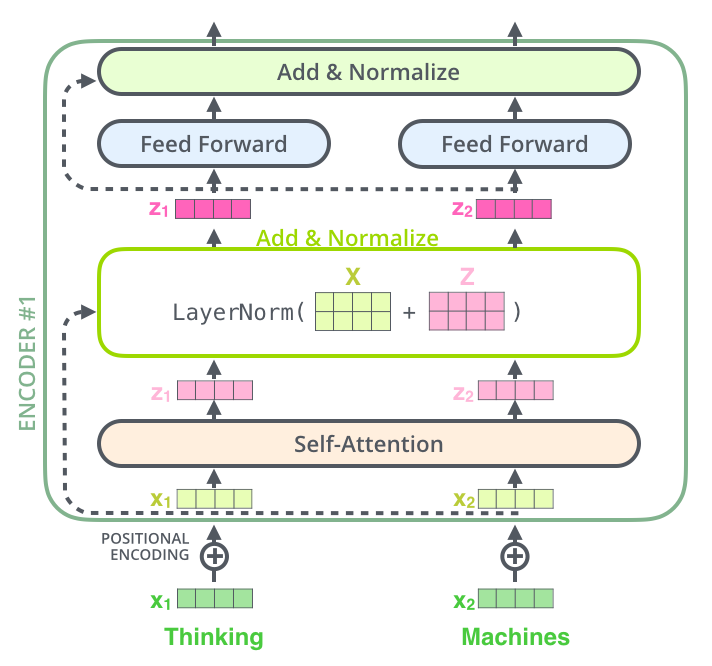
\includegraphics[scale=0.3]{pics/transformer_resideual_layer_norm_2.png}
\end{figure}


\section{El codificador: resumen}

\begin{figure}[h]
  \centering
  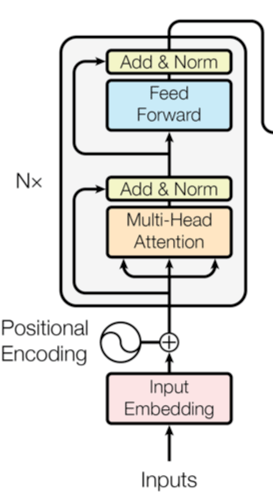
\includegraphics[scale=0.39]{pics/transformerencoder.png}
\end{figure}

Lo que hace cada bloque codificador es, en realidad, una serie de multiplicaciones de matrices seguidas de un par de transformaciones elemento a elemento. Es por eso que el Transformer es tan rápido: todo se reduce a multiplicaciones de matrices paralelizables. El punto es que, apilando estas transformaciones una encima de la otra, podemos crear una red muy potente. El núcleo de esto es el mecanismo de atención, que modifica y atiende una amplia gama de información.



\section{El Decodificador}

El decodificador del Transformer consta de dos tipos de capas de atención: atención propia y atención codificador-decodificador. Las capas de atención propia en el decodificador permiten que cada posición en el decodificador preste atención a todas las posiciones dentro del propio decodificador, de manera similar a cómo funciona el estado oculto en las arquitecturas de traducción de máquinas RNN.  Por otro lado, la capa de ``atención codificador-decodificador'' permite que el decodificador se enfoque en partes relevantes de la secuencia de entrada.

La capa de atención codificador-decodificador funciona de manera similar a la atención propia de múltiples cabezas, pero genera su matriz de consultas a partir de la capa inferior y utiliza las matrices de claves y valores de la salida de la pila del codificador. Esto permite que cada posición en el decodificador atienda a todas las posiciones en la secuencia de entrada, imitando los mecanismos de atención codificador-decodificador típicos vistos en los modelos de secuencia a secuencia RNN.

\begin{figure}[h]
  \centering
  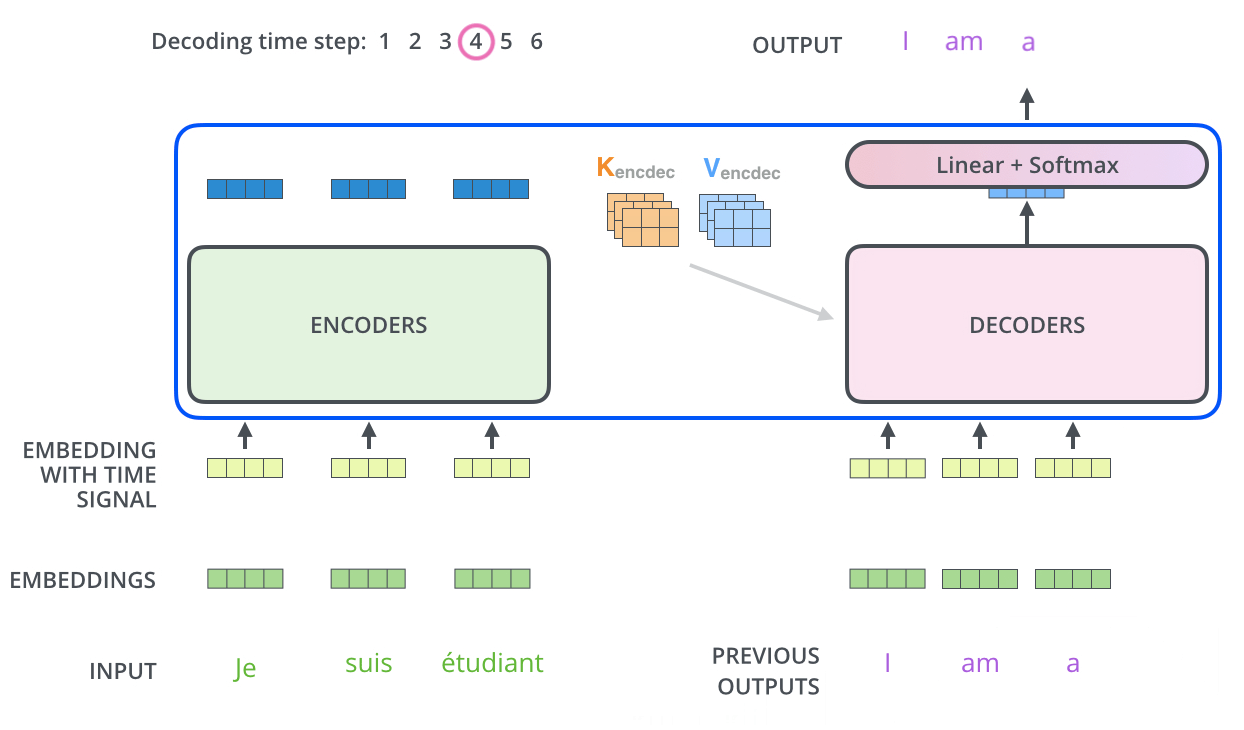
\includegraphics[scale=0.28]{pics/transformer_decoder.png}
\end{figure}

Cada paso en la fase de decodificación produce un elemento de la secuencia de salida (la oración de traducción al inglés en este caso). Este proceso se repite hasta que se alcanza un símbolo especial que indica que el decodificador del Transformer ha completado su salida. Cuando entrenamos el Transformer, queremos procesar todas las oraciones al mismo tiempo.

Sin embargo, si le damos al decodificador acceso a toda la oración de destino, el modelo puede simplemente repetir la oración de destino (en otras palabras, no necesita aprender nada). La capa de atención propia solo debe poder atender a las posiciones anteriores en la secuencia de salida. Esto se logra enmascarando los tokens ``futuros'' al decodificar una palabra determinada.

El enmascaramiento se realiza estableciendo en $- \infty$ todos los valores en la entrada de la función softmax que corresponden a conexiones ilegales. Es por eso que los ``bloques de atención propia'' en el decodificador se llaman ``enmascarados'': las entradas al decodificador de pasos de tiempo futuros están enmascaradas.


\begin{figure}[h]
  \centering
  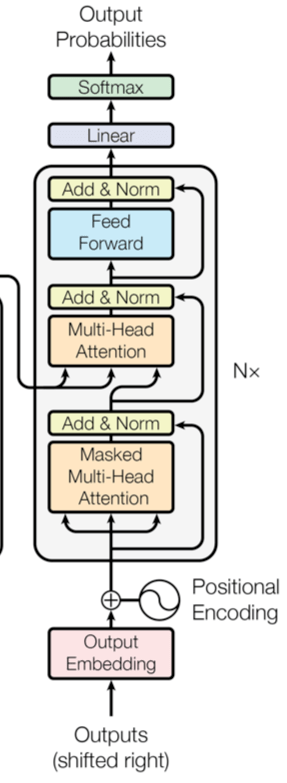
\includegraphics[scale=0.29]{pics/transformerdecoder.png}
\end{figure}

\section{La Capa Lineal Final y el Entrenamiento}
La pila del decodificador genera un vector de números reales como su salida. Para convertir este vector en una palabra, se utiliza la capa lineal final, seguida de una capa softmax. La capa lineal es una red neuronal completamente conectada que proyecta el vector de salida del decodificador en un vector más grande llamado vector de logits. El vector de logits tiene una dimensión igual al tamaño del vocabulario de salida del modelo, que contiene 10,000 palabras en inglés únicas. Cada celda del vector de logits representa la puntuación de una palabra específica.  La capa softmax luego transforma estas puntuaciones en probabilidades, asegurándose de que todas sean positivas y sumen 1.0.

\begin{figure}[h]
  \centering
  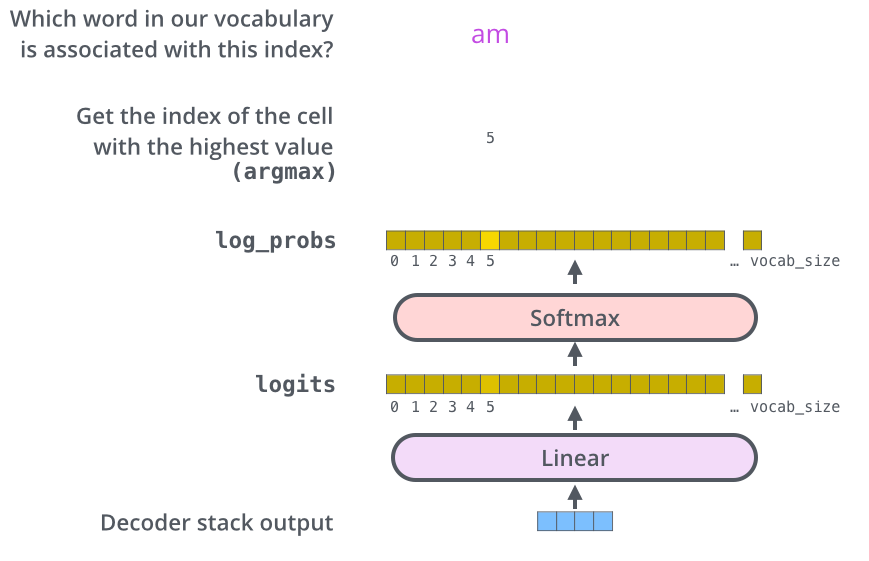
\includegraphics[scale=0.2]{pics/transformer_decoder_output_softmax.png}
\end{figure}

La palabra con la probabilidad más alta se elige como la salida para el paso de tiempo actual. Durante el entrenamiento del Transformer, se utiliza una pérdida de entropía cruzada.Esta pérdida mide la diferencia entre la distribución de palabras predicha y la palabra objetivo, que se representa como un vector one-hot.



\section{Codificaciones posicionales}


A diferencia de las redes recurrentes, la red de atención múltiple no puede utilizar de manera natural la posición de las palabras en la secuencia de entrada. Sin codificaciones posicionales, la salida de la red de atención múltiple sería la misma para las oraciones ``I like cats more than dogs'' y ``I like dogs more than cats''.

Las codificaciones posicionales codifican explícitamente las posiciones relativas/absolutas de las entradas como vectores y luego se suman a las incrustaciones de entrada.

\begin{figure}[h]
  \centering
  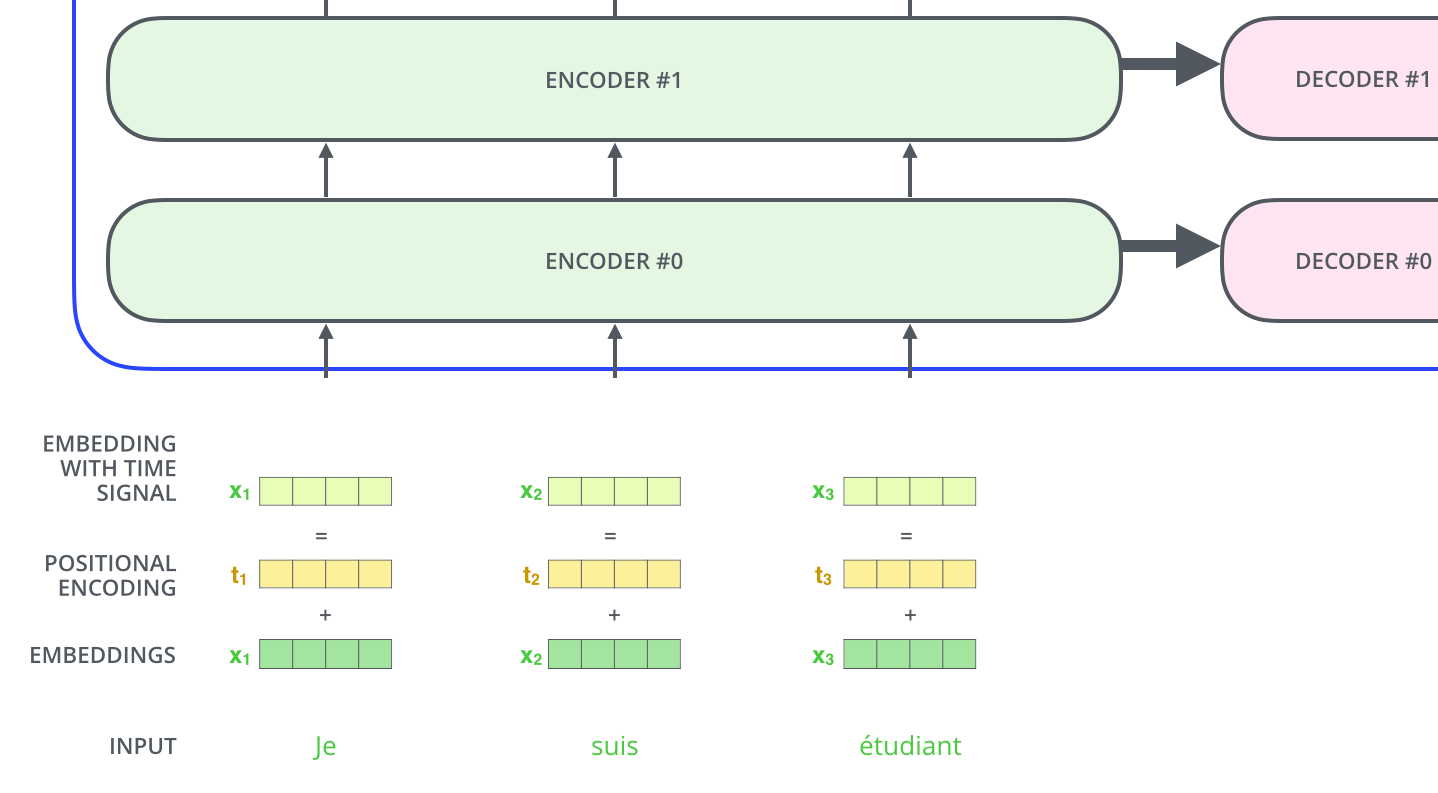
\includegraphics[scale=0.2]{pics/transformer_positional_encoding_vectors.png}
\end{figure}

Para darle al modelo una idea del orden de las palabras, agregamos vectores de codificación posicional, cuyos valores siguen un patrón específico.

El documento utiliza la siguiente ecuación para calcular las codificaciones posicionales:\\
$PE(pos,2i) = \sin(pos/10000^{2i/d_{model}})$
$PE(pos,2i+1) = \cos(pos/10000^{2i/d_{model}})$

Donde $pos$ representa la posición, e $i$ es la dimensión. Básicamente, cada dimensión de la codificación posicional es una onda con una frecuencia diferente.

\begin{figure}[h]
  \centering
  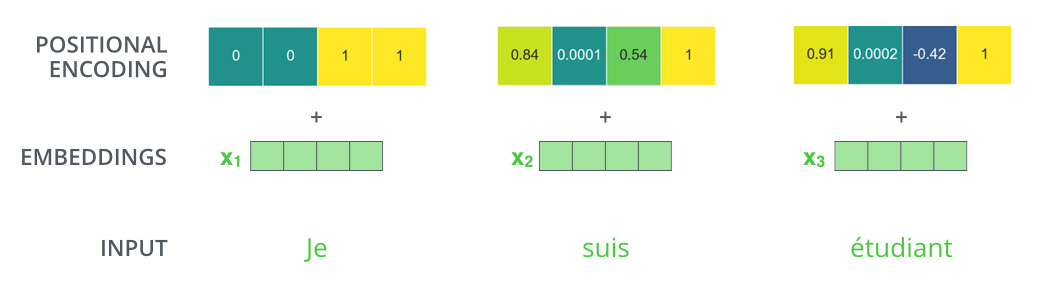
\includegraphics[scale=0.25]{pics/transformer_positional_encoding_example.png}
\end{figure}

Un ejemplo real de codificación posicional con un tamaño de incrustación de juguete de 4.


\section{Conclusiones}

El Transformer logra mejores puntuaciones BLEU que los modelos anteriores del estado del arte para la traducción del inglés al alemán y del inglés al francés a una fracción del costo de entrenamiento.

\begin{figure}[h]
  \centering
  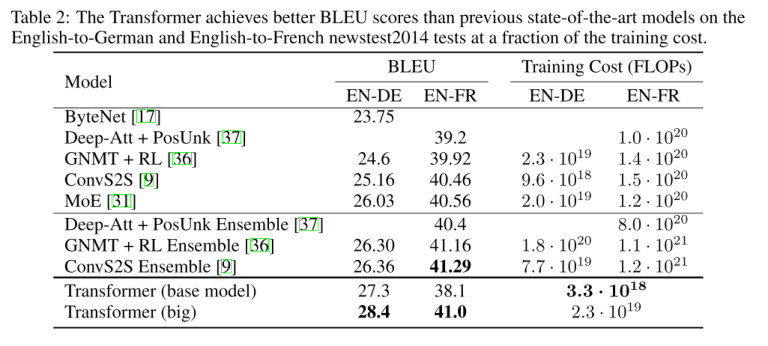
\includegraphics[scale=0.29]{pics/transformerresults.png}
\end{figure}

El Transformer es una alternativa potente y eficiente a las redes neuronales recurrentes para modelar dependencias utilizando solo mecanismos de atención.

Se ha establecido como la arquitectura de facto en el procesamiento del lenguaje natural y sirve como base para los modelos de lenguaje grandes y modernos.

